\documentclass{beamer}

\usepackage[utf8]{inputenc}
\usepackage{graphicx}
\graphicspath{ {./images/} }
\usetheme{Warsaw}
%\usecolortheme{beaver}

%Information to be included in the title page:
\title[About Beamer] %optional
{About the Beamer class in presentation making}
\subtitle{A short story}
\author[Arthur, Doe] % (optional, for multiple authors)
{A.~B.~Arthur\inst{1} \and J.~Doe\inst{2}}
\institute[VFU] % (optional)
{
  \inst{1}%
  Faculty of Physics\\
  Very Famous University
  \and
  \inst{2}%
  Faculty of Chemistry\\
  Very Famous University
}

\date[VLC 2013] % (optional)
{Very Large Conference, April 2013}



\begin{document}

\frame{\titlepage}

\begin{frame}
\frametitle{Sample frame title}
This is a text in the first frame. This is a text in the first frame. This is a text in the first frame.
\end{frame}

\begin{frame}
 Aqui voy a poner las ideas principales de la plática \pause

texto \pause

Presentar una lo que es una L-linea, describir el problema, primero resolver parcialmente el problema con los arboles,i.e ,describir la construccion de las poligonos, ortognales, espirales, contruccion del arbol, decir porque se forma un arbol, pasar a la tranformacion de los 3 arboles a trayectorias, y mencionar el trabajo que despues se hizo (revisar las referencias del capitulo de libro de mikio kano)
\end{frame}
\begin{figure}[b]
\begin{center}
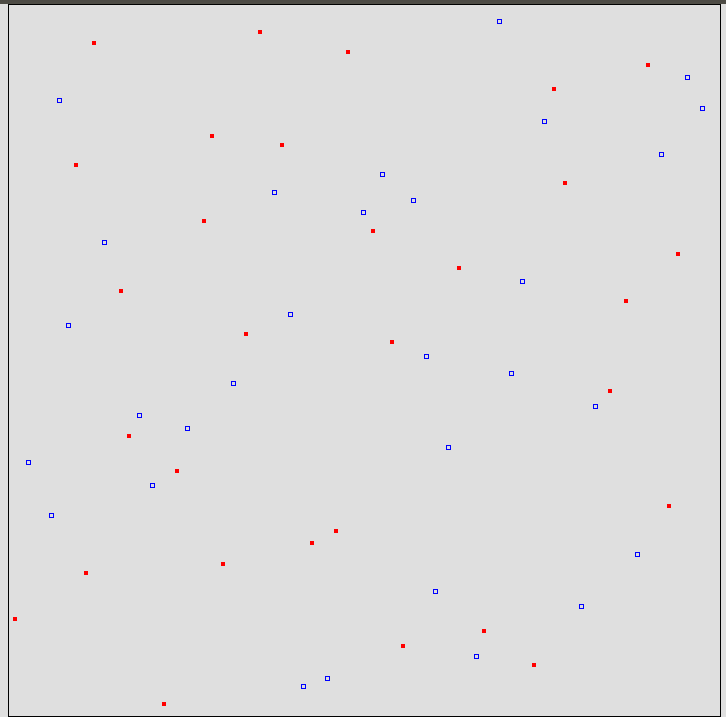
\includegraphics[width=6cm, height=6cm]{n-puntos}
\end{center}
\end{figure}


\end{document}